\chapter{提案手法}

\section{A*アルゴリズムの概要}

A*アルゴリズムは、グラフ探索における最短経路探索アルゴリズムとして広く知られている。A*は、始点から終点までの最適経路を効率的に探索するため、各ノードに対して評価関数を計算し、最も有望なノードから優先的に探索を進める。この探索戦略により、無駄な探索を削減し、効率的に最短経路を発見できる。

A*における各ノード$n$の評価関数$f(n)$は、以下の式で定義される。

\begin{equation}
f(n) = g(n) + h(n)
\label{eq:4_astar_basic}
\end{equation}

ここで、$g(n)$は始点からノード$n$までの実コスト（既知のコスト）、$h(n)$はノード$n$からゴールまでの推定コスト（ヒューリスティック関数）である。A*は、$f(n)$が最小となるノードを優先的に展開することで、効率的に最短経路を探索する。

ヒューリスティック関数$h(n)$は、ノード$n$からゴールまでの推定コストを表す。一般的に、2次元グリッド環境では、ユークリッド距離やマンハッタン距離が用いられる。ヒューリスティック関数が許容的（真のコストを過大評価しない）である場合、A*は最適解を保証する。本研究では、ユークリッド距離をベースとしたヒューリスティック関数を採用した。

A*のアルゴリズムは、オープンリストとクローズドリストの2つのデータ構造を用いる。オープンリストは、未探索のノードを格納し、評価関数$f(n)$の小さい順にソートされる。クローズドリストは、既に探索済みのノードを格納する。A*は、オープンリストから$f(n)$が最小のノードを取り出し、そのノードの隣接ノードを展開する。展開されたノードは、オープンリストに追加され、探索が繰り返される。ゴールノードがクローズドリストに追加されると、探索は終了し、最短経路が得られる。

\section{既存手法の問題点}

式(\ref{eq:4_astar_basic})の通常のA*アルゴリズムは、始点からゴールまでの経路長を最小化することを目的としている。しかし、この評価関数は地形の特性（傾斜、粗さ、障害物密度など）を考慮していない。そのため、不整地環境においては、最短経路が必ずしも走行しやすい経路とは限らない。

例えば、始点とゴールの間に丘がある場合、通常のA*は丘を直線的に越える最短経路を選択する。しかし、急斜面を登ることはロボットの走行安定性を損なう可能性があり、消費エネルギーも増大する。一方、丘を迂回する経路は距離は長くなるが、平坦な地形を走行できるため、安全かつ効率的である。このように、不整地環境では、経路長だけでなく地形の特性を考慮した経路計画が必要となる。

\subsection{関連する既存手法}

評価関数に複数のコスト項を導入する手法として、weighted A*や多目的A*が知られている。weighted A*は、ヒューリスティック関数に重みを付けることで探索の速度と最適性のトレードオフを制御する手法である。多目的A*は、経路長以外の複数の評価基準（エネルギー消費、安全性など）を統合した経路計画を行う手法である。

これらの既存手法は、評価関数に複数の要素を組み込むという点で本研究と共通している。しかし、以下の点で本研究は既存手法と異なる独自性を持つ。

\subsection{本研究の独自性}

本研究の独自性は、以下の3点にある。

\textbf{（1）リアルタイム点群データからの地形コスト計算：}
既存の多くの地形考慮型経路計画手法は、事前に作成された地形マップや、特定の地形要因（傾斜のみ、など）に限定されている。本研究では、RTAB-Mapというリアルタイム3次元SLAM技術から得られる点群データを用いて、標高差、傾斜角、表面粗さの3要素を統合した地形複雑度を計算する。この統合により、実用的なセンサーシステムから直接、包括的な地形評価が可能となる。

\textbf{（2）実装可能性の高いシステム統合：}
アルゴリズム単体としては、本研究の評価関数はweighted A*の一種と見なすこともできる。しかし、本研究の貢献は、RTAB-Mapという実用的なSLAMツールと経路計画アルゴリズムを統合し、点群取得から経路生成までの一貫したシステムとして提案している点にある。この統合により、実環境での実装可能性が高いシステムを構築している。

\textbf{（3）2つの評価方法による多角的評価：}
地形コストの評価において、点平均法（アルゴリズムの地形回避能力を評価）とセグメント加重法（実際の移動コストを評価）という2つの評価方法を導入し、それぞれの役割を明確化した。これにより、アルゴリズムの設計意図と実用的な性能を分離して評価できる。

以上の独自性により、本研究は単なる既存手法の組み合わせではなく、実用的な地形考慮型自律移動システムの構築に貢献する。

\section{Terrain-Aware A*の提案}

本研究では、地形情報を考慮した経路計画手法としてTerrain-Aware A*（TA*）を提案する。TA*は、通常のA*アルゴリズムを拡張し、評価関数に地形コストを統合することで、不整地環境において安全かつ効率的な経路を生成する。これにより、経路長だけでなく、地形複雑度も考慮した総合的な経路評価が可能となる。

TA*における評価関数は、通常のA*の評価関数に地形コスト項を加算する形で定義する：

\begin{equation}
f(n) = g(n) + h(n) + w_t \times t(n)
\label{eq:4_ta_astar}
\end{equation}

ここで、$w_t$は地形コストと経路長の相対的重要度を表すパラメータである。$w_t$を大きくすると地形回避を重視し、小さくすると経路長を重視する。$g(n)$と$h(n)$は経路長に関するコスト[m]であるのに対し、$t(n)$は地形複雑度（無次元量）であり、次元が異なる。そのため、$w_t$の値自体に直接的な物理的意味はなく、実験的に最適値を決定する必要がある。本研究では、予備実験により$w_t = 1.0$が経路長と地形品質のバランスにおいて良好であることを確認した。

各項の役割を詳しく説明する。$g(n)$は始点からノード$n$までの累積移動コストであり、実際に移動した距離に基づいて計算される。$h(n)$はノード$n$からゴールまでのユークリッド距離を用いたヒューリスティック関数である。$t(n)$は地形コストであり、第3章の式(\ref{eq:3_terrain_cost})で定義した地形コストを用いる。$w_t$は地形重みパラメータであり、環境の特性やロボットの性能に応じて調整される。$w_t$を大きくすると地形回避を重視し、小さくすると経路長を重視する。

TA*のアルゴリズムは、通常のA*と同様に、オープンリストとクローズドリストを用いる。唯一の違いは、評価関数に地形コスト項が追加されることである。これにより、地形の良いノードが優先的に選択され、地形の悪い領域を回避する経路が生成される。

\section{地形コストの計算}

ノード$n$の地形コスト$t(n)$は、第3章で定義した地形複雑度$T_c(n)$を最大値$T_c^{max}$で正規化することで計算される。

\begin{equation}
t(n) = \frac{T_c(n)}{T_c^{max}}
\label{eq:4_terrain_cost}
\end{equation}

ここで、$T_c(n)$は式(\ref{eq:3_terrain_complexity})で計算されたノード$n$の地形複雑度、$T_c^{max}$は環境内の全ノードにおける地形複雑度の最大値である。この正規化により、地形コストは0から1の範囲に収まり、他のコスト項とのバランスが取りやすくなる。

経路全体の地形品質を評価するため、経路上の各ノードの地形コストを累積する。本研究では、2つの評価方法を用いた。第一の方法（点平均法）は、経路上の各ノードの地形コストの平均値である。この方法は、経路がどの程度地形の良い領域を通過しているかを直接的に表す。

\begin{equation}
C_{avg} = \frac{1}{N} \sum_{i=1}^{N} t(n_i)
\label{eq:4_point_average}
\end{equation}

ここで、$N$は経路上のノード数、$n_i$は$i$番目のノードである。

第二の方法（セグメント加重法）は、各セグメント（ノード間の移動）の距離に応じて地形コストを加重平均する。この方法は、実際の移動コストにより近い評価を行える。

\begin{equation}
C_{seg} = \frac{\sum_{i=1}^{N-1} d_i \cdot t(n_i)}{\sum_{i=1}^{N-1} d_i}
\label{eq:4_segment_weighted}
\end{equation}

ここで、$d_i$はノード$n_i$と$n_{i+1}$の間の距離である。本研究では、主にセグメント加重法を用いて評価を行った。

\section{パラメータ調整}

地形重み$w_t$は、経路長と地形回避のバランスを制御する重要なパラメータである。$w_t$を小さく設定すると、式(\ref{eq:4_ta_astar})において$g(n)$と$h(n)$の影響が大きくなり、通常のA*に近い動作となる。つまり、経路長を重視した探索が行われる。一方、$w_t$を大きく設定すると、$t(n)$の影響が大きくなり、地形の良いノードが優先的に選択される。ただし、$w_t$を過度に大きくすると、探索ノード数が爆発的に増加し、計算時間が増大する問題がある。

本研究では、予備実験により$w_t$を0.0から2.0まで0.2刻みで変化させ、hill\_detourシナリオにおける経路品質を評価した。図\ref{fig:wt_tuning}に$w_t$と各性能指標の関係を示す。

\begin{figure}[htbp]
\centering
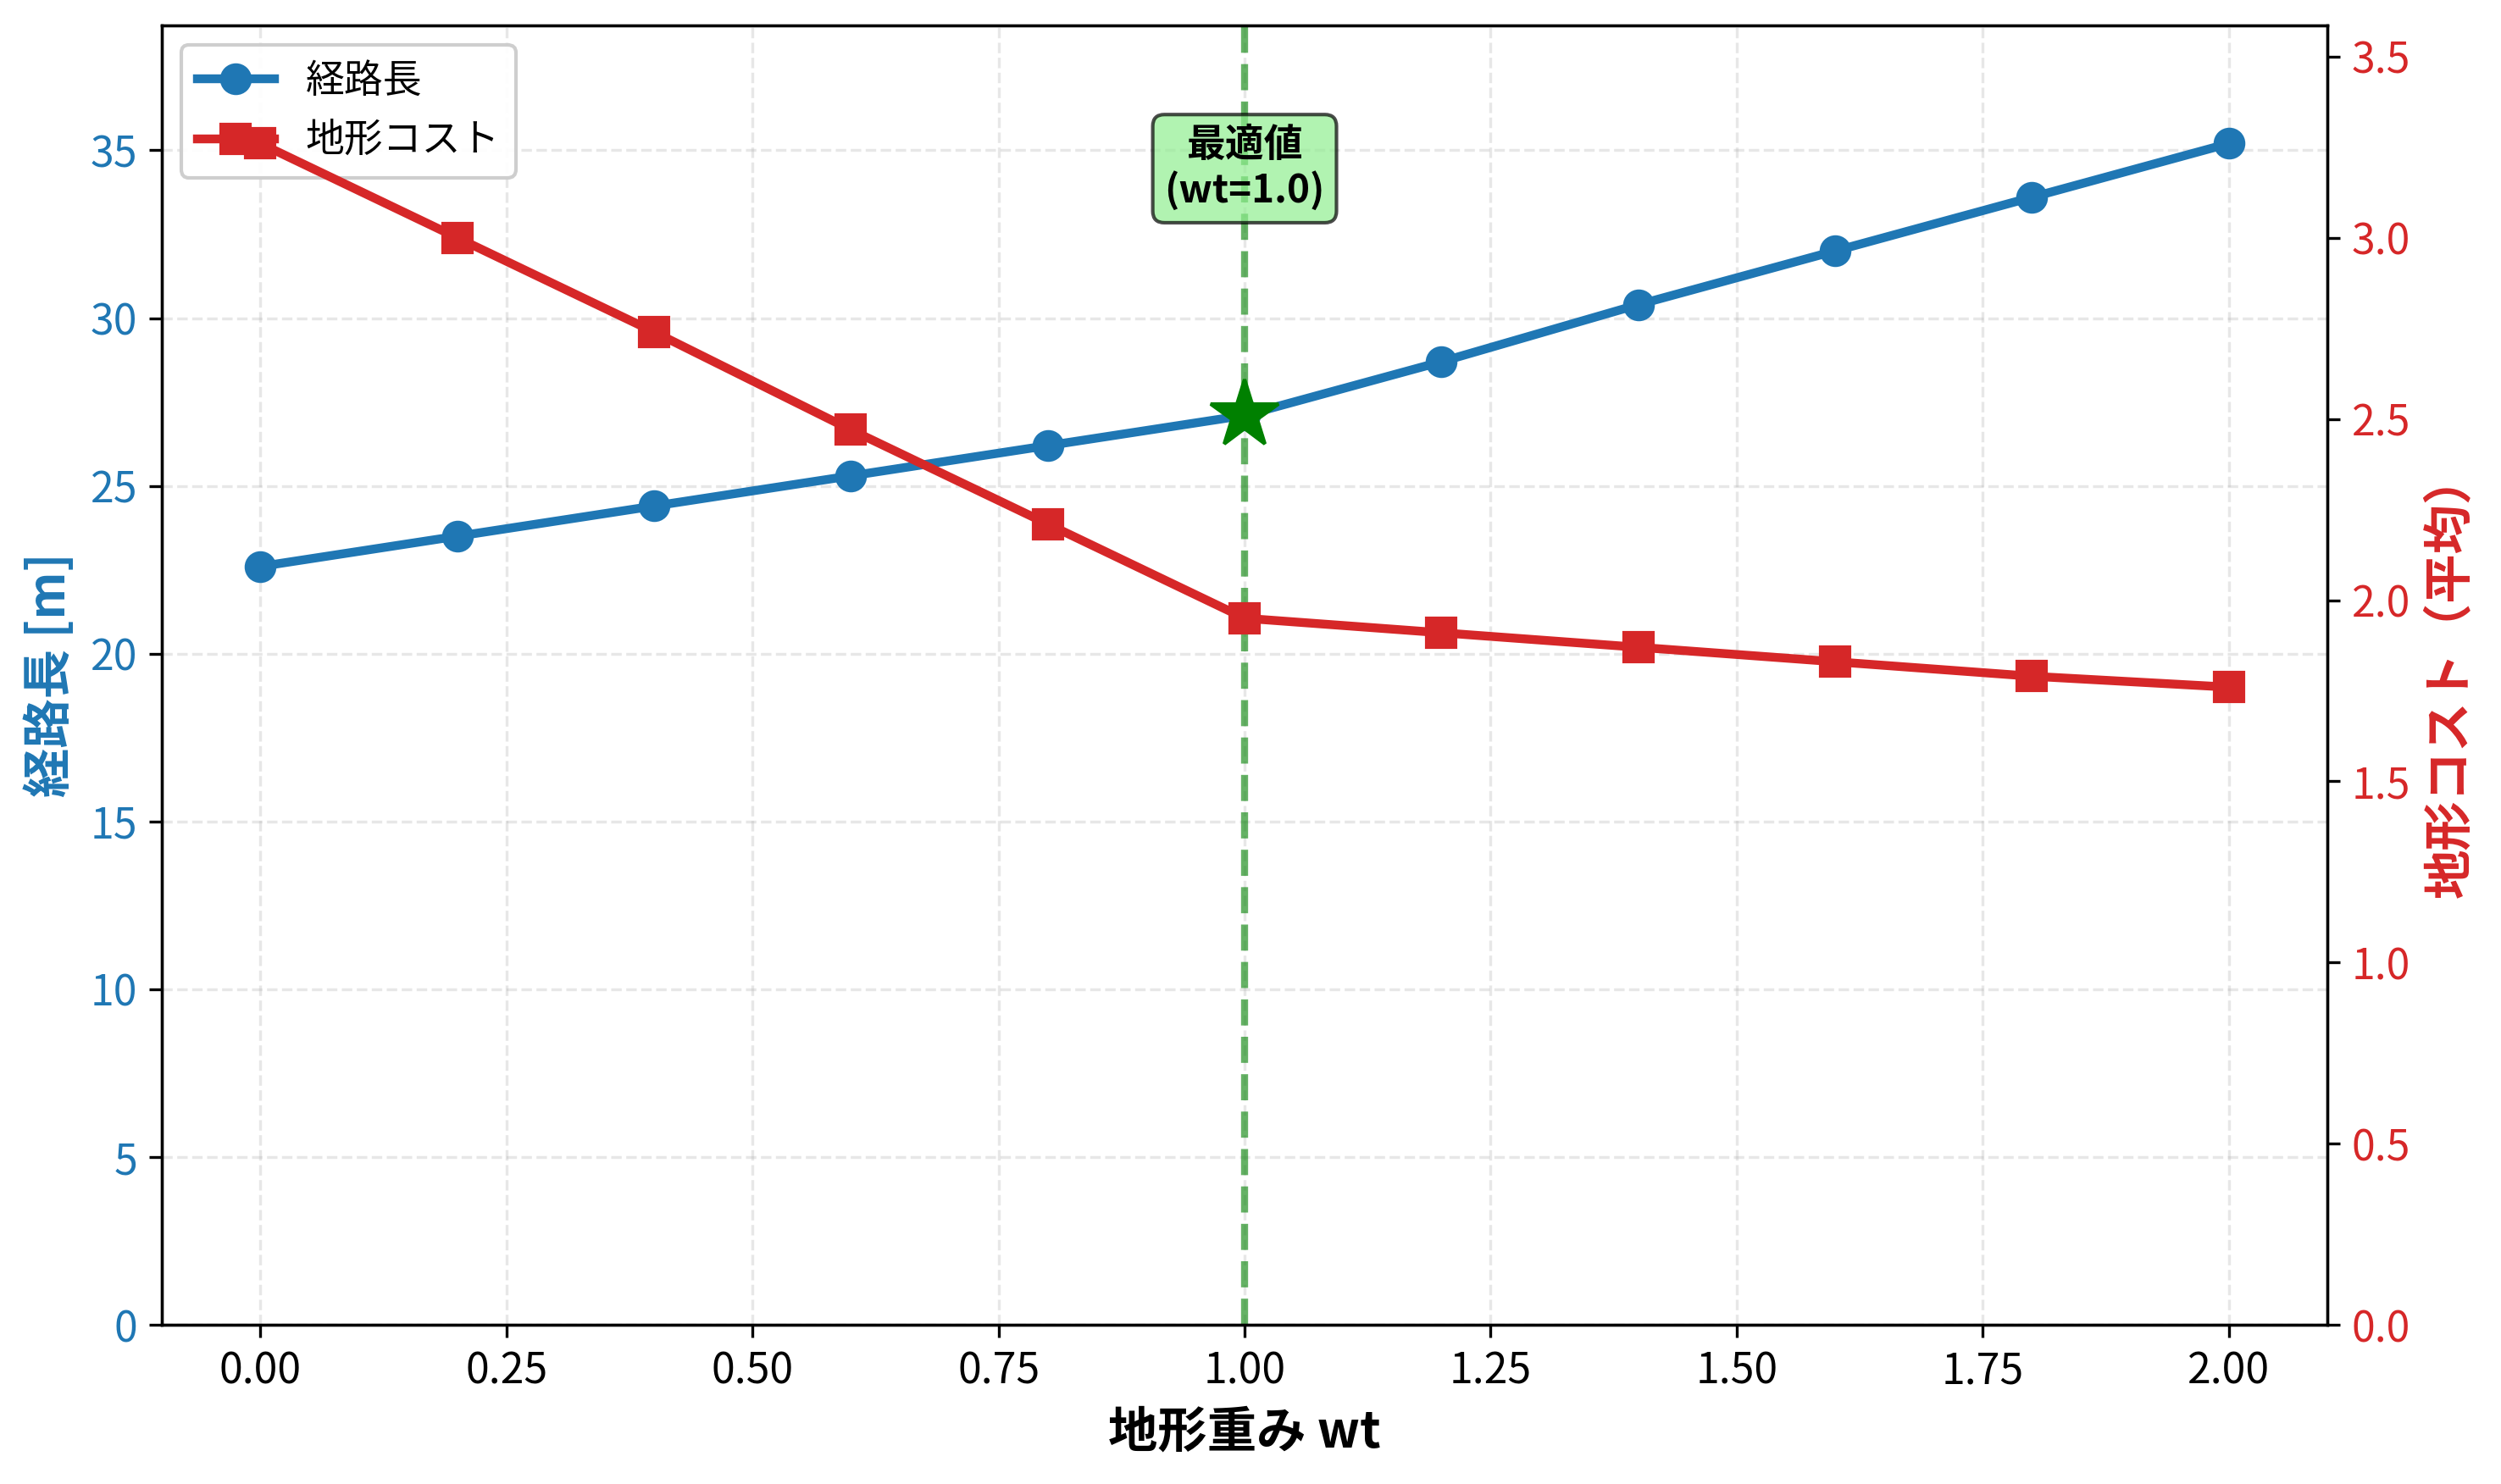
\includegraphics[width=\textwidth,height=0.6\textheight,keepaspectratio]{figures/fig_wt_parameter_tuning.png}
\caption{地形重み$w_t$と性能指標の関係（hill\_detourシナリオ）}
\label{fig:wt_tuning}
\end{figure}

$w_t = 0.8$では地形コストの削減が不十分（約32\%削減）であり、地形回避能力が限定的であった。一方、$w_t = 1.2$では計算時間が12.7秒に増加し、実時間性が低下する結果となった。$w_t = 1.0$では、点平均法による地形コストを40.3\%削減しながら、経路長の増加を19.7\%に抑え、かつ計算時間も約9秒と許容範囲内に収まった。これらの結果から、$w_t = 1.0$が経路長、地形品質、計算時間の3要素のバランスにおいて最良であると判断し、本実験ではこの値を採用した。

$w_t$の選択は、ロボットの性能や環境の特性に依存する。登坂能力の高いロボットでは、$w_t$を小さく設定し、経路長を重視することができる。一方、登坂能力の低いロボットや、安全性を重視する用途では、$w_t$を大きく設定し、地形回避を優先することが望ましい。実用上は、現場の状況に応じて動的に$w_t$を調整することも考えられる。

\section{Field D* Hybridとの統合}

Field D*は、D*アルゴリズムの拡張版であり、隣接セル間で補間を行うことで、グリッドベースの制約を緩和する手法である。通常のグリッドベースのアルゴリズムでは、経路がグリッドのエッジに沿って生成されるため、不自然な折れ曲がりが生じる。Field D*は、隣接セル間で補間を行うことで、グリッドに制約されない滑らかな経路を生成できる。これにより、経路長を短縮し、より自然なロボットの動きを実現できる。

本研究では、TA*の評価関数にField D*の補間技術を統合したField D* Hybridを開発した。Field D* Hybridは、以下の手順でField D*の補間技術とTA*の評価関数を統合する。

\textbf{（1）補間点候補の生成：}
通常のField D*と同様に、各ノード$n$の隣接セルについて補間点候補を生成する。具体的には、ノード$n$から隣接セルの各エッジ上の点を候補として考慮する。

\textbf{（2）地形コストの補間計算：}
各補間点$p$に対して、その位置における地形コスト$t(p)$を双線形補間により計算する。補間点$p$が4つのグリッド点$(x_1, y_1), (x_2, y_1), (x_1, y_2), (x_2, y_2)$に囲まれている場合、それぞれの地形コスト$t(x_1, y_1), t(x_2, y_1), t(x_1, y_2), t(x_2, y_2)$を用いて、以下の双線形補間により$t(p)$を計算する：

\begin{equation}
t(p) = (1-u)(1-v)t(x_1,y_1) + u(1-v)t(x_2,y_1) + (1-u)v t(x_1,y_2) + uv t(x_2,y_2)
\end{equation}

ここで、$(u,v)$は補間点$p$の正規化座標（$0 \leq u,v \leq 1$）である。具体的には、$p$の位置を$(x,y)$とすると、$u = \frac{x - x_1}{x_2 - x_1}$、$v = \frac{y - y_1}{y_2 - y_1}$により計算される。

\textbf{（3）評価関数によるコスト計算：}
各補間点$p$に対して、TA*の評価関数(式\ref{eq:4_ta_astar})を用いてコストを計算する：
\begin{equation}
f(p) = g(p) + h(p) + w_t \times t(p)
\end{equation}

ここで、$g(p)$はスタートから補間点$p$までの実コスト、$h(p)$は補間点$p$からゴールまでの推定コスト、$t(p)$は双線形補間により計算された地形コストである。

\textbf{（4）最適経由点の選択：}
$f(p)$が最小となる補間点を最適経由点として選択し、次の探索ノードとする。

この統合により、グリッド制約を緩和しながら地形考慮も実現できる。すなわち、Field D* Hybridは、Field D*の経路平滑化能力とTA*の地形回避能力を同時に活用することで、短く滑らかで、かつ地形の良い経路を生成する。

Field D* Hybridの性能評価結果については第6章で詳述する。

\section{アルゴリズムのフロー}

TA*のアルゴリズムは、以下の流れで実行される。まず、スタートノードをオープンリストに追加し、$g(start) = 0$、$f(start) = h(start) + w_t \times t(start)$と初期化する。次に、オープンリストから$f(n)$が最小のノード$n$を取り出し、クローズドリストに移動する。ノード$n$がゴールノードであれば、探索を終了し、経路を復元する。

ノード$n$がゴールでない場合、ノード$n$の隣接ノードについて、以下の処理を行う。隣接ノード$n'$が障害物である場合、スキップする。$n'$がクローズドリストに含まれる場合、スキップする。$n'$までの新しいコスト$g_{new} = g(n) + c(n, n')$を計算する。ここで、$c(n, n')$はノード$n$から$n'$への移動コストである。

$n'$がオープンリストに含まれない場合、$g(n') = g_{new}$、$f(n') = g(n') + h(n') + w_t \times t(n')$として、$n'$をオープンリストに追加する。$n'$が既にオープンリストに含まれ、$g_{new} < g(n')$の場合、$g(n')$と$f(n')$を更新する。

この処理を、オープンリストが空になるか、ゴールに到達するまで繰り返す。ゴールに到達した場合、各ノードの親ノードを辿ることで、経路を復元する。

TA*のアルゴリズムフローを示す。

\section{まとめ}

本章では、A*アルゴリズムの基本原理、既存手法の問題点と本研究の独自性、および地形コストを導入したTerrain-Aware A*（TA*）を提案した。本研究の独自性は、RTAB-Mapから得られるリアルタイム点群データを用いた地形コスト計算と、実装可能性の高いシステム統合にある。TA*は、通常のA*の評価関数に地形コスト項を追加することで、不整地環境において安全な経路を生成する。地形重みパラメータ$w_t$を調整することで、経路長と地形品質のバランスを制御できる。

また、Field D*の補間技術を統合したField D* Hybridを開発し、経路平滑化と地形考慮を同時に実現する手法を提案した。Field D* Hybridは、双線形補間により補間点の地形コストを計算し、TA*の評価関数により最適経由点を選択する。次章では、これらの提案手法の実験的評価について述べる。